\section{LowLevelPacket Class Reference}
\label{classLowLevelPacket}\index{LowLevelPacket@{LowLevelPacket}}
{\tt \#include $<$lowLevelPacket.h$>$}

Collaboration diagram for LowLevelPacket:\nopagebreak
\begin{figure}[H]
\begin{center}
\leavevmode
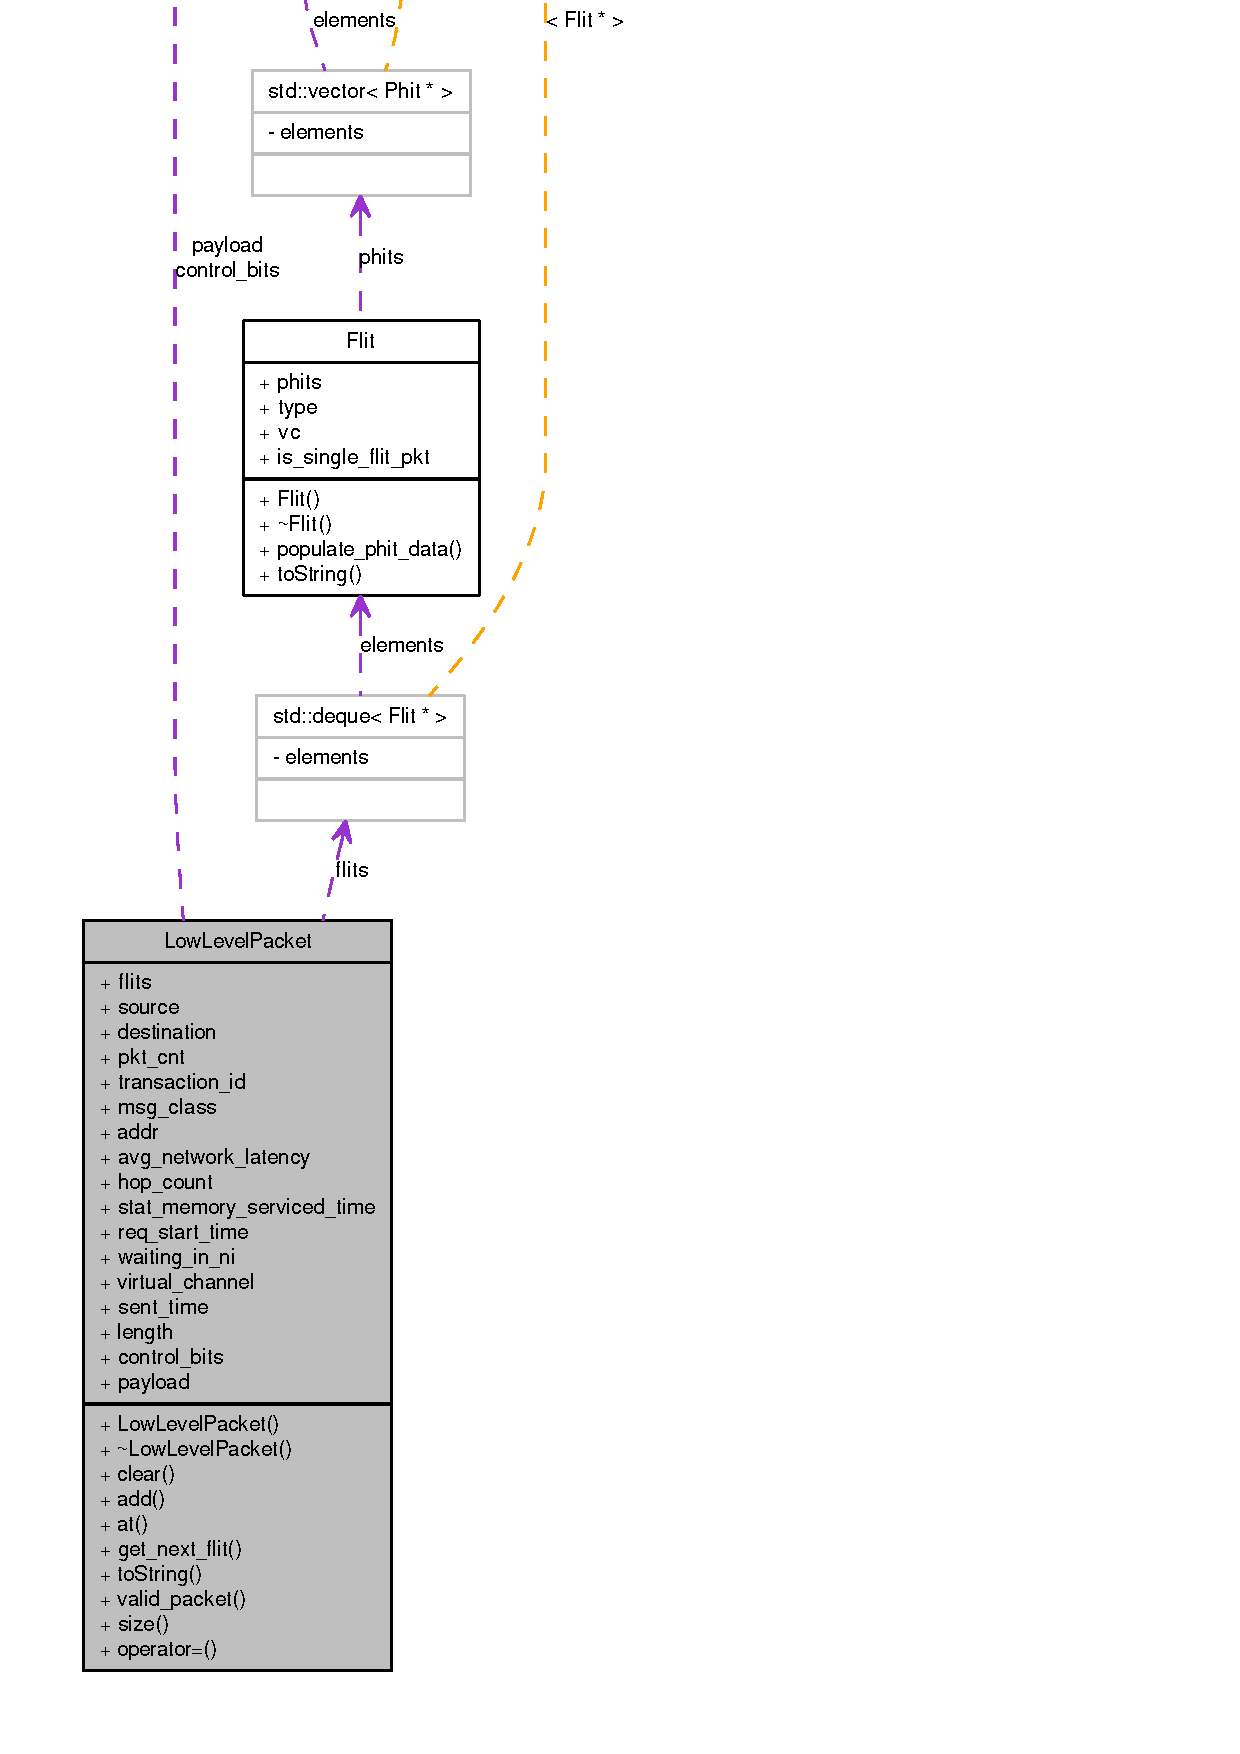
\includegraphics[height=400pt]{classLowLevelPacket__coll__graph}
\end{center}
\end{figure}
\subsection*{Public Member Functions}
\begin{CompactItemize}
\item 
{\bf LowLevelPacket} ()
\item 
{\bf $\sim$LowLevelPacket} ()
\item 
void {\bf clear} ()
\item 
void {\bf add} ({\bf Flit} $\ast$ptr)
\item 
{\bf Flit} $\ast$ {\bf at} ({\bf uint} index)
\item 
{\bf Flit} $\ast$ {\bf get\_\-next\_\-flit} ()
\item 
string {\bf toString} () const 
\item 
bool {\bf valid\_\-packet} ()
\item 
{\bf uint} {\bf size} ()
\item 
void {\bf operator=} (const {\bf LowLevelPacket} $\ast$p)
\end{CompactItemize}
\subsection*{Public Attributes}
\begin{CompactItemize}
\item 
deque$<$ {\bf Flit} $\ast$ $>$ {\bf flits}
\item 
{\bf uint} {\bf source}
\item 
{\bf uint} {\bf destination}
\item 
{\bf uint} {\bf pkt\_\-cnt}
\item 
{\bf uint} {\bf transaction\_\-id}
\item 
{\bf message\_\-class} {\bf msg\_\-class}
\item 
{\bf ullint} {\bf addr}
\item 
double {\bf avg\_\-network\_\-latency}
\item 
unsigned int {\bf hop\_\-count}
\item 
unsigned int {\bf stat\_\-memory\_\-serviced\_\-time}
\item 
{\bf ullint} {\bf req\_\-start\_\-time}
\item 
{\bf ullint} {\bf waiting\_\-in\_\-ni}
\item 
short int {\bf virtual\_\-channel}
\item 
unsigned long int {\bf sent\_\-time}
\item 
unsigned int {\bf length}
\item 
vector$<$ bool $>$ {\bf control\_\-bits}
\item 
vector$<$ bool $>$ {\bf payload}
\end{CompactItemize}


\subsection{Detailed Description}


Definition at line 45 of file lowLevelPacket.h.

\subsection{Constructor \& Destructor Documentation}
\index{LowLevelPacket@{LowLevelPacket}!LowLevelPacket@{LowLevelPacket}}
\index{LowLevelPacket@{LowLevelPacket}!LowLevelPacket@{LowLevelPacket}}
\subsubsection[{LowLevelPacket}]{\setlength{\rightskip}{0pt plus 5cm}LowLevelPacket::LowLevelPacket ()}\label{classLowLevelPacket_550561f33ccae00163b40e963121c156}




Definition at line 27 of file lowLevelPacket.cc.

References destination, length, sent\_\-time, source, transaction\_\-id, and virtual\_\-channel.\index{LowLevelPacket@{LowLevelPacket}!$\sim$LowLevelPacket@{$\sim$LowLevelPacket}}
\index{$\sim$LowLevelPacket@{$\sim$LowLevelPacket}!LowLevelPacket@{LowLevelPacket}}
\subsubsection[{$\sim$LowLevelPacket}]{\setlength{\rightskip}{0pt plus 5cm}LowLevelPacket::$\sim$LowLevelPacket ()}\label{classLowLevelPacket_52d6041c394872c42cd4211e09ca76d4}




Definition at line 38 of file lowLevelPacket.cc.

References control\_\-bits, flits, and payload.

\subsection{Member Function Documentation}
\index{LowLevelPacket@{LowLevelPacket}!add@{add}}
\index{add@{add}!LowLevelPacket@{LowLevelPacket}}
\subsubsection[{add}]{\setlength{\rightskip}{0pt plus 5cm}void LowLevelPacket::add ({\bf Flit} $\ast$ {\em ptr})}\label{classLowLevelPacket_b2d005a02fb4645db9145f699d330656}




Definition at line 104 of file lowLevelPacket.cc.

References HeadFlit::addr, addr, TailFlit::avg\_\-network\_\-latency, HeadFlit::avg\_\-network\_\-latency, avg\_\-network\_\-latency, BodyFlit::bf\_\-data, BODY, control\_\-bits, HeadFlit::control\_\-bits, destination, HeadFlit::dst\_\-address, HEAD, HeadFlit::hop\_\-count, hop\_\-count, HeadFlit::length, length, HeadFlit::msg\_\-class, msg\_\-class, TailFlit::packet\_\-originated\_\-time, HeadFlit::packet\_\-originated\_\-time, payload, HeadFlit::payload, HeadFlit::pkt\_\-cnt, pkt\_\-cnt, HeadFlit::req\_\-start\_\-time, req\_\-start\_\-time, sent\_\-time, source, HeadFlit::src\_\-address, HeadFlit::stat\_\-memory\_\-serviced\_\-time, stat\_\-memory\_\-serviced\_\-time, TAIL, HeadFlit::transaction\_\-id, transaction\_\-id, Flit::type, Flit::vc, virtual\_\-channel, HeadFlit::waiting\_\-in\_\-ni, and waiting\_\-in\_\-ni.\index{LowLevelPacket@{LowLevelPacket}!at@{at}}
\index{at@{at}!LowLevelPacket@{LowLevelPacket}}
\subsubsection[{at}]{\setlength{\rightskip}{0pt plus 5cm}{\bf Flit} $\ast$ LowLevelPacket::at ({\bf uint} {\em index})}\label{classLowLevelPacket_01bcea53e1afb4be73ddaa8503e053dc}




Definition at line 161 of file lowLevelPacket.cc.

References flits.\index{LowLevelPacket@{LowLevelPacket}!clear@{clear}}
\index{clear@{clear}!LowLevelPacket@{LowLevelPacket}}
\subsubsection[{clear}]{\setlength{\rightskip}{0pt plus 5cm}void LowLevelPacket::clear ()}\label{classLowLevelPacket_726a1d04c62dc4f20de1bcd7bebd031d}




Definition at line 178 of file lowLevelPacket.cc.

References flits.\index{LowLevelPacket@{LowLevelPacket}!get\_\-next\_\-flit@{get\_\-next\_\-flit}}
\index{get\_\-next\_\-flit@{get\_\-next\_\-flit}!LowLevelPacket@{LowLevelPacket}}
\subsubsection[{get\_\-next\_\-flit}]{\setlength{\rightskip}{0pt plus 5cm}{\bf Flit} $\ast$ LowLevelPacket::get\_\-next\_\-flit ()}\label{classLowLevelPacket_508b439358881368b5ef646ef36b4cac}




Definition at line 169 of file lowLevelPacket.cc.

References flits.\index{LowLevelPacket@{LowLevelPacket}!operator=@{operator=}}
\index{operator=@{operator=}!LowLevelPacket@{LowLevelPacket}}
\subsubsection[{operator=}]{\setlength{\rightskip}{0pt plus 5cm}void LowLevelPacket::operator= (const {\bf LowLevelPacket} $\ast$ {\em p})}\label{classLowLevelPacket_5a52c8b9499a757227a71ba51f1ef61a}




Definition at line 45 of file lowLevelPacket.cc.

References control\_\-bits, destination, length, msg\_\-class, payload, pkt\_\-cnt, sent\_\-time, source, transaction\_\-id, and virtual\_\-channel.\index{LowLevelPacket@{LowLevelPacket}!size@{size}}
\index{size@{size}!LowLevelPacket@{LowLevelPacket}}
\subsubsection[{size}]{\setlength{\rightskip}{0pt plus 5cm}{\bf uint} LowLevelPacket::size ()}\label{classLowLevelPacket_f61b1051a4dbda237dbeb1bd74220d20}




Definition at line 185 of file lowLevelPacket.cc.

References flits.\index{LowLevelPacket@{LowLevelPacket}!toString@{toString}}
\index{toString@{toString}!LowLevelPacket@{LowLevelPacket}}
\subsubsection[{toString}]{\setlength{\rightskip}{0pt plus 5cm}string LowLevelPacket::toString (void) const}\label{classLowLevelPacket_5a52563bae0560cb9b0b9a6d44adde6c}




Definition at line 63 of file lowLevelPacket.cc.

References addr, avg\_\-network\_\-latency, destination, flits, hop\_\-count, length, msg\_\-class, pkt\_\-cnt, sent\_\-time, source, and virtual\_\-channel.\index{LowLevelPacket@{LowLevelPacket}!valid\_\-packet@{valid\_\-packet}}
\index{valid\_\-packet@{valid\_\-packet}!LowLevelPacket@{LowLevelPacket}}
\subsubsection[{valid\_\-packet}]{\setlength{\rightskip}{0pt plus 5cm}bool LowLevelPacket::valid\_\-packet ()}\label{classLowLevelPacket_1053348a061e1878e90a4f49d383889f}




Definition at line 94 of file lowLevelPacket.cc.

References flits, and length.

\subsection{Member Data Documentation}
\index{LowLevelPacket@{LowLevelPacket}!addr@{addr}}
\index{addr@{addr}!LowLevelPacket@{LowLevelPacket}}
\subsubsection[{addr}]{\setlength{\rightskip}{0pt plus 5cm}{\bf ullint} {\bf LowLevelPacket::addr}}\label{classLowLevelPacket_c7767df59c8c88c21171828b30f2b176}




Definition at line 59 of file lowLevelPacket.h.

Referenced by add(), HighLevelPacket::from\_\-low\_\-level\_\-packet(), HighLevelPacket::to\_\-low\_\-level\_\-packet(), and toString().\index{LowLevelPacket@{LowLevelPacket}!avg\_\-network\_\-latency@{avg\_\-network\_\-latency}}
\index{avg\_\-network\_\-latency@{avg\_\-network\_\-latency}!LowLevelPacket@{LowLevelPacket}}
\subsubsection[{avg\_\-network\_\-latency}]{\setlength{\rightskip}{0pt plus 5cm}double {\bf LowLevelPacket::avg\_\-network\_\-latency}}\label{classLowLevelPacket_9b6dc1d5e9944a52c17037ea6fd5d729}




Definition at line 62 of file lowLevelPacket.h.

Referenced by add(), HighLevelPacket::from\_\-low\_\-level\_\-packet(), HighLevelPacket::to\_\-low\_\-level\_\-packet(), and toString().\index{LowLevelPacket@{LowLevelPacket}!control\_\-bits@{control\_\-bits}}
\index{control\_\-bits@{control\_\-bits}!LowLevelPacket@{LowLevelPacket}}
\subsubsection[{control\_\-bits}]{\setlength{\rightskip}{0pt plus 5cm}vector$<$bool$>$ {\bf LowLevelPacket::control\_\-bits}}\label{classLowLevelPacket_7537b9b0339e77d3d4a2d04998e1a950}




Definition at line 71 of file lowLevelPacket.h.

Referenced by add(), HighLevelPacket::from\_\-low\_\-level\_\-packet(), operator=(), HighLevelPacket::to\_\-low\_\-level\_\-packet(), and $\sim$LowLevelPacket().\index{LowLevelPacket@{LowLevelPacket}!destination@{destination}}
\index{destination@{destination}!LowLevelPacket@{LowLevelPacket}}
\subsubsection[{destination}]{\setlength{\rightskip}{0pt plus 5cm}{\bf uint} {\bf LowLevelPacket::destination}}\label{classLowLevelPacket_225808b46aefe4d252c040e91c9411b0}




Definition at line 54 of file lowLevelPacket.h.

Referenced by add(), HighLevelPacket::from\_\-low\_\-level\_\-packet(), LowLevelPacket(), operator=(), HighLevelPacket::to\_\-low\_\-level\_\-packet(), and toString().\index{LowLevelPacket@{LowLevelPacket}!flits@{flits}}
\index{flits@{flits}!LowLevelPacket@{LowLevelPacket}}
\subsubsection[{flits}]{\setlength{\rightskip}{0pt plus 5cm}deque$<${\bf Flit}$\ast$$>$ {\bf LowLevelPacket::flits}}\label{classLowLevelPacket_eee86f15c92fad6be8b7e6bc4df223e3}




Definition at line 52 of file lowLevelPacket.h.

Referenced by at(), clear(), HighLevelPacket::from\_\-low\_\-level\_\-packet(), get\_\-next\_\-flit(), size(), HighLevelPacket::to\_\-low\_\-level\_\-packet(), toString(), valid\_\-packet(), and $\sim$LowLevelPacket().\index{LowLevelPacket@{LowLevelPacket}!hop\_\-count@{hop\_\-count}}
\index{hop\_\-count@{hop\_\-count}!LowLevelPacket@{LowLevelPacket}}
\subsubsection[{hop\_\-count}]{\setlength{\rightskip}{0pt plus 5cm}unsigned int {\bf LowLevelPacket::hop\_\-count}}\label{classLowLevelPacket_33d231de5104e9f1a79c4b313e8ab5c6}




Definition at line 63 of file lowLevelPacket.h.

Referenced by add(), HighLevelPacket::from\_\-low\_\-level\_\-packet(), HighLevelPacket::to\_\-low\_\-level\_\-packet(), and toString().\index{LowLevelPacket@{LowLevelPacket}!length@{length}}
\index{length@{length}!LowLevelPacket@{LowLevelPacket}}
\subsubsection[{length}]{\setlength{\rightskip}{0pt plus 5cm}unsigned int {\bf LowLevelPacket::length}}\label{classLowLevelPacket_69297a63b62cdce301d004782cc3ef3c}




Definition at line 70 of file lowLevelPacket.h.

Referenced by add(), HighLevelPacket::from\_\-low\_\-level\_\-packet(), LowLevelPacket(), operator=(), HighLevelPacket::to\_\-low\_\-level\_\-packet(), toString(), and valid\_\-packet().\index{LowLevelPacket@{LowLevelPacket}!msg\_\-class@{msg\_\-class}}
\index{msg\_\-class@{msg\_\-class}!LowLevelPacket@{LowLevelPacket}}
\subsubsection[{msg\_\-class}]{\setlength{\rightskip}{0pt plus 5cm}{\bf message\_\-class} {\bf LowLevelPacket::msg\_\-class}}\label{classLowLevelPacket_f910145223e23da0d8d5fca5b231cd9a}




Definition at line 57 of file lowLevelPacket.h.

Referenced by add(), HighLevelPacket::from\_\-low\_\-level\_\-packet(), operator=(), HighLevelPacket::to\_\-low\_\-level\_\-packet(), and toString().\index{LowLevelPacket@{LowLevelPacket}!payload@{payload}}
\index{payload@{payload}!LowLevelPacket@{LowLevelPacket}}
\subsubsection[{payload}]{\setlength{\rightskip}{0pt plus 5cm}vector$<$bool$>$ {\bf LowLevelPacket::payload}}\label{classLowLevelPacket_aef0f881df6e8d70d2db8f8810a98a51}




Definition at line 72 of file lowLevelPacket.h.

Referenced by add(), HighLevelPacket::from\_\-low\_\-level\_\-packet(), operator=(), and $\sim$LowLevelPacket().\index{LowLevelPacket@{LowLevelPacket}!pkt\_\-cnt@{pkt\_\-cnt}}
\index{pkt\_\-cnt@{pkt\_\-cnt}!LowLevelPacket@{LowLevelPacket}}
\subsubsection[{pkt\_\-cnt}]{\setlength{\rightskip}{0pt plus 5cm}{\bf uint} {\bf LowLevelPacket::pkt\_\-cnt}}\label{classLowLevelPacket_b4fcaaaddcb7d0e82671adfa3e2c4a44}




Definition at line 55 of file lowLevelPacket.h.

Referenced by add(), HighLevelPacket::from\_\-low\_\-level\_\-packet(), operator=(), HighLevelPacket::to\_\-low\_\-level\_\-packet(), and toString().\index{LowLevelPacket@{LowLevelPacket}!req\_\-start\_\-time@{req\_\-start\_\-time}}
\index{req\_\-start\_\-time@{req\_\-start\_\-time}!LowLevelPacket@{LowLevelPacket}}
\subsubsection[{req\_\-start\_\-time}]{\setlength{\rightskip}{0pt plus 5cm}{\bf ullint} {\bf LowLevelPacket::req\_\-start\_\-time}}\label{classLowLevelPacket_1520729379478975bb4132437027c434}




Definition at line 65 of file lowLevelPacket.h.

Referenced by add(), HighLevelPacket::from\_\-low\_\-level\_\-packet(), and HighLevelPacket::to\_\-low\_\-level\_\-packet().\index{LowLevelPacket@{LowLevelPacket}!sent\_\-time@{sent\_\-time}}
\index{sent\_\-time@{sent\_\-time}!LowLevelPacket@{LowLevelPacket}}
\subsubsection[{sent\_\-time}]{\setlength{\rightskip}{0pt plus 5cm}unsigned long int {\bf LowLevelPacket::sent\_\-time}}\label{classLowLevelPacket_8a51892863d89c8b8b28f75c19fa0199}




Definition at line 69 of file lowLevelPacket.h.

Referenced by add(), HighLevelPacket::from\_\-low\_\-level\_\-packet(), LowLevelPacket(), operator=(), HighLevelPacket::to\_\-low\_\-level\_\-packet(), and toString().\index{LowLevelPacket@{LowLevelPacket}!source@{source}}
\index{source@{source}!LowLevelPacket@{LowLevelPacket}}
\subsubsection[{source}]{\setlength{\rightskip}{0pt plus 5cm}{\bf uint} {\bf LowLevelPacket::source}}\label{classLowLevelPacket_c7aee6df6db0e4bb8e5be36b061a95bc}




Definition at line 53 of file lowLevelPacket.h.

Referenced by add(), HighLevelPacket::from\_\-low\_\-level\_\-packet(), LowLevelPacket(), operator=(), HighLevelPacket::to\_\-low\_\-level\_\-packet(), and toString().\index{LowLevelPacket@{LowLevelPacket}!stat\_\-memory\_\-serviced\_\-time@{stat\_\-memory\_\-serviced\_\-time}}
\index{stat\_\-memory\_\-serviced\_\-time@{stat\_\-memory\_\-serviced\_\-time}!LowLevelPacket@{LowLevelPacket}}
\subsubsection[{stat\_\-memory\_\-serviced\_\-time}]{\setlength{\rightskip}{0pt plus 5cm}unsigned int {\bf LowLevelPacket::stat\_\-memory\_\-serviced\_\-time}}\label{classLowLevelPacket_b8f013b92fcf6f6caa2bd5c9d1cecf31}




Definition at line 64 of file lowLevelPacket.h.

Referenced by add(), HighLevelPacket::from\_\-low\_\-level\_\-packet(), and HighLevelPacket::to\_\-low\_\-level\_\-packet().\index{LowLevelPacket@{LowLevelPacket}!transaction\_\-id@{transaction\_\-id}}
\index{transaction\_\-id@{transaction\_\-id}!LowLevelPacket@{LowLevelPacket}}
\subsubsection[{transaction\_\-id}]{\setlength{\rightskip}{0pt plus 5cm}{\bf uint} {\bf LowLevelPacket::transaction\_\-id}}\label{classLowLevelPacket_ed8dd9d70bac87be59a61fe8ac4b399d}




Definition at line 56 of file lowLevelPacket.h.

Referenced by add(), HighLevelPacket::from\_\-low\_\-level\_\-packet(), LowLevelPacket(), operator=(), and HighLevelPacket::to\_\-low\_\-level\_\-packet().\index{LowLevelPacket@{LowLevelPacket}!virtual\_\-channel@{virtual\_\-channel}}
\index{virtual\_\-channel@{virtual\_\-channel}!LowLevelPacket@{LowLevelPacket}}
\subsubsection[{virtual\_\-channel}]{\setlength{\rightskip}{0pt plus 5cm}short int {\bf LowLevelPacket::virtual\_\-channel}}\label{classLowLevelPacket_3fa4ac5563bbf3005a809c0b193f4c84}




Definition at line 68 of file lowLevelPacket.h.

Referenced by add(), HighLevelPacket::from\_\-low\_\-level\_\-packet(), LowLevelPacket(), operator=(), HighLevelPacket::to\_\-low\_\-level\_\-packet(), and toString().\index{LowLevelPacket@{LowLevelPacket}!waiting\_\-in\_\-ni@{waiting\_\-in\_\-ni}}
\index{waiting\_\-in\_\-ni@{waiting\_\-in\_\-ni}!LowLevelPacket@{LowLevelPacket}}
\subsubsection[{waiting\_\-in\_\-ni}]{\setlength{\rightskip}{0pt plus 5cm}{\bf ullint} {\bf LowLevelPacket::waiting\_\-in\_\-ni}}\label{classLowLevelPacket_d6a9b48c6d2c4576519fa38e8166b356}




Definition at line 66 of file lowLevelPacket.h.

Referenced by add(), and HighLevelPacket::from\_\-low\_\-level\_\-packet().

The documentation for this class was generated from the following files:\begin{CompactItemize}
\item 
{\bf lowLevelPacket.h}\item 
{\bf lowLevelPacket.cc}\end{CompactItemize}
